% !TeX program = xelatex
\documentclass[a4paper,10pt]{article}

% ============================================================================
% សន្លឹកកិច្ចការសិស្ស ស-ខ្មៅ (Student Guided-Inquiry Worksheet - Grade 8 15.3 CIRC3)
% បរិបទ៖ គ្មានស្លាយ LCD — សិស្សប្រើបន្ទាត់ក្រិតវាស់អង្កត់ធ្នូលើរូបខ្នាតពិត 1:1 និងបំពេញសម្រាយបញ្ជាក់
% វិធីសាស្ត្រ៖ POE (1:1 Ruler Chord Inquiry) + Backward-Faded Proof Worksheet
% ============================================================================
\usepackage[a4paper, left=1.0cm, right=1.0cm, top=0.80cm, bottom=1.00cm, footskip=0.50cm]{geometry}
\usepackage{amsmath, amssymb}
\usepackage{unicode-math}
\usepackage{fontspec}
\usepackage{array, colortbl}
\usepackage[table]{xcolor}
\usepackage{enumitem}
\usepackage{pifont}
\usepackage{fancyhdr}
\usepackage{lastpage}
\usepackage{tikz}
\usepackage[most]{tcolorbox}
\usetikzlibrary{calc, arrows.meta, angles, quotes, decorations.markings, positioning, babel}

\makeatletter
\let\@expl@@@mark@update@singlecol@structures@@\relax
\makeatother

\providecommand{\NGSFindFonts}{%
  \IfFileExists{C:/Windows/Fonts/cambria.ttc}{%
    \def\NGSSysPath{C:/Windows/Fonts/}%
    \def\NGSUserPath{C:/Users/KIT/AppData/Local/Microsoft/Windows/Fonts/}%
  }{%
    \IfFileExists{./fonts/KhmerOSsiemreap.ttf}{\def\NGSSysPath{./fonts/}\def\NGSUserPath{./fonts/}}{%
    \IfFileExists{../fonts/KhmerOSsiemreap.ttf}{\def\NGSSysPath{../fonts/}\def\NGSUserPath{../fonts/}}{%
    \IfFileExists{../../fonts/KhmerOSsiemreap.ttf}{\def\NGSSysPath{../../fonts/}\def\NGSUserPath{../../fonts/}}{%
    \IfFileExists{../../../fonts/KhmerOSsiemreap.ttf}{\def\NGSSysPath{../../../fonts/}\def\NGSUserPath{../../../fonts/}}{%
    \IfFileExists{../../../../fonts/KhmerOSsiemreap.ttf}{\def\NGSSysPath{../../../../fonts/}\def\NGSUserPath{../../../../fonts/}}{%
    \IfFileExists{../../../../../fonts/KhmerOSsiemreap.ttf}{\def\NGSSysPath{../../../../../fonts/}\def\NGSUserPath{../../../../../fonts/}}{%
    \IfFileExists{../../../../../../fonts/KhmerOSsiemreap.ttf}{\def\NGSSysPath{../../../../../../fonts/}\def\NGSUserPath{../../../../../../fonts/}}{%
      \def\NGSSysPath{../../../../../../../fonts/}\def\NGSUserPath{../../../../../../../fonts/}%
    }}}}}}}%
  }%
}
\NGSFindFonts

\setmathfont[Path={\NGSSysPath}, FontIndex=1, Scale=1.02]{cambria.ttc}
\defaultfontfeatures{Ligatures=TeX}

\setmainfont[
  Path={\NGSUserPath}, Extension=.ttf, Script=Khmer,
  BoldFont={KhmerOSsiemreap}, BoldFeatures={FakeBold=1.8},
  ItalicFont={KhmerOSsiemreap}, ItalicFeatures={FakeSlant=0.25},
  BoldItalicFont={KhmerOSsiemreap}, BoldItalicFeatures={FakeBold=1.8, FakeSlant=0.25}
]{KhmerOSsiemreap}

\newfontfamily\muol[Path={\NGSUserPath}, Extension=.ttf, Script=Khmer]{KhmerOSmuollight}
\newfontfamily\TimesEn[Path={\NGSSysPath}, Extension=.ttf, BoldFont={timesbd}, ItalicFont={timesi}, BoldItalicFont={timesbi}]{times}
\newfontfamily\CalibriFont[Path={\NGSSysPath}, Extension=.ttf]{calibri}

\XeTeXlinebreaklocale "km"
\XeTeXlinebreakskip = 0pt plus 1pt minus 0.1pt

\definecolor{panelgray}{gray}{0.93}
\definecolor{headgray}{gray}{0.85}

\pagestyle{fancy}
\fancyhf{}
\renewcommand{\headrulewidth}{0pt}
\fancyfoot[L]{\fontsize{8.0pt}{10pt}\selectfont អនុវិទ្យាល័យព្រះក្រសាំង \en{|} គណិតវិទ្យា ថ្នាក់ទី៨ \en{---} មេរៀនទី១៥ (២.២ ធ្នូ និងអង្កត់ធ្នូ) \en{|} គ្រូបង្រៀន៖ ហុក ប៊ុនថែន}
\fancyfoot[R]{\fontsize{8.2pt}{10pt}\selectfont ទំព័រ \en{\thepage\ / \pageref{LastPage}}}

\setlength{\parindent}{0pt}
\setlength{\parskip}{0pt}
\setlength{\tabcolsep}{4pt}

\newcommand{\en}[1]{{\TimesEn #1}}
\newcommand{\enbf}[1]{{\TimesEn\bfseries #1}}
\newcommand{\unit}[1]{\,\text{\en{#1}}}
\newcommand{\cnum}[1]{\mbox{\fontsize{10pt}{12pt}\selectfont\ding{\numexpr181+#1\relax}}}
\newcommand{\chkbox}{\tikz[baseline=-0.15ex]\draw[black, line width=0.85pt] (0,0) rectangle (0.24cm,0.24cm);}
\newcommand{\tri}[1]{\ensuremath{\triangle #1}}
\newcommand{\ang}[1]{\ensuremath{\angle #1}}
\newcommand{\arc}[1]{\ensuremath{\overset{\tikz[baseline=-0.55ex]\draw[black, line width=0.55pt] (0,0) to[bend left=40] (1.8ex,0);}{#1}}}
\newcommand{\blank}[1]{\underline{\hspace{#1}}}

\newcommand{\secbox}[2]{%
  \begin{tcolorbox}[
    enhanced, sharp corners, colback=headgray, colframe=black,
    boxrule=0.95pt, boxsep=1pt, top=2.0pt, bottom=2.0pt, left=6pt, right=6pt,
    before skip=3pt, after skip=2pt
  ]
    {\muol\fontsize{9.2pt}{13.2pt}\selectfont #1}\hfill{\fontsize{8.2pt}{11.5pt}\selectfont\textbf{#2}}
  \end{tcolorbox}%
}

\newcolumntype{L}[1]{>{\raggedright\arraybackslash}p{#1}}
\newcolumntype{C}[1]{>{\centering\arraybackslash}p{#1}}

\begin{document}
\fontsize{9.2pt}{13.6pt}\selectfont

% ============================================================================
% ទំព័រទី ១ ៖ ក្បាលសន្លឹកកិច្ចការ + ផ្នែក ក (E2 POE 1:1) + ផ្នែក ខ (E3 ទ្រឹស្ដីបទ & ធនាគារហេតុផល)
% ============================================================================
\begin{tcolorbox}[
  enhanced, sharp corners, colback=white, colframe=black,
  boxrule=1.1pt, boxsep=2pt, top=3pt, bottom=3pt, left=6pt, right=6pt, after skip=3pt
]
  \begin{minipage}[c]{12.2cm}
    {\muol\fontsize{10.8pt}{15pt}\selectfont សន្លឹកកិច្ចការសិស្ស ១៥.៣ ៖ ធ្នូ និងអង្កត់ធ្នូនៃរង្វង់}\\[2pt]
    ឈ្មោះសិស្ស៖ \blank{4.2cm}\quad ក្រុមទី៖ \blank{1.1cm}\quad ថ្នាក់ទី៨៖ \blank{1.2cm}\\[2pt]
    \textbf{បេសកកម្មជាងឈើ \en{E1}៖} អង្កត់ធ្នូវែងបំផុតគឺ \blank{2.2cm} \en{|} មុំកើន $60^\circ \to 120^\circ$ អង្កត់ធ្នូកើនទ្វេដងឬទេ? \chkbox\ បាទ/ចាស \;\chkbox\ ទេ
  \end{minipage}\hfill%
  \begin{minipage}[c]{5.8cm}
    \centering
    {\fontsize{7.6pt}{9.5pt}\selectfont\textbf{បន្ទះផ្ទៀងខ្នាតពិត \en{5.00 cm (Actual Size 100\%)}}}\\[1pt]
    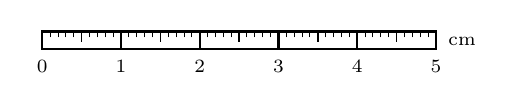
\begin{tikzpicture}[x=1cm, y=1cm]
      \draw[black, line width=0.9pt] (0,0) rectangle (5.0,0.22);
      \foreach \x in {0,1,2,3,4,5} {
        \draw[black, line width=0.8pt] (\x,0) -- (\x,0.22);
        \node[below=0.5pt, font=\fontsize{6.8pt}{8pt}\selectfont] at (\x,0) {\en{\x}};
      }
      \foreach \x in {0.5,1.5,2.5,3.5,4.5} {
        \draw[black, line width=0.6pt] (\x,0.09) -- (\x,0.22);
      }
      \foreach \x in {0.1,0.2,0.3,0.4,0.6,0.7,0.8,0.9,1.1,1.2,1.3,1.4,1.6,1.7,1.8,1.9,2.1,2.2,2.3,2.4,2.6,2.7,2.8,2.9,3.1,3.2,3.3,3.4,3.6,3.7,3.8,3.9,4.1,4.2,4.3,4.4,4.6,4.7,4.8,4.9} {
        \draw[black, line width=0.35pt] (\x,0.15) -- (\x,0.22);
      }
      \node[right=1pt, font=\fontsize{6.8pt}{8pt}\selectfont] at (5.0,0.10) {\en{cm}};
    \end{tikzpicture}
  \end{minipage}
\end{tcolorbox}

% -------------------- ផ្នែក ក (E2 Explore - POE) --------------------
\secbox{ផ្នែក ក \enbf{(E2 Explore - POE)} ៖ ពិសោធន៍វាស់អង្កត់ធ្នូលើរង្វង់ខ្នាតពិត \enbf{1:1} ($r = 2.20\unit{cm}$)}{១១ នាទី \en{---} ប្រើបន្ទាត់ក្រិតមីលីម៉ែត្រ}

\begin{minipage}[t]{7.5cm}
  \vspace{0pt}
  \begin{tcolorbox}[
    enhanced, sharp corners, colback=white, colframe=black,
    boxrule=0.8pt, boxsep=1pt, top=2pt, bottom=2pt, left=2pt, right=2pt
  ]
    \centering
    {\fontsize{8.0pt}{10pt}\selectfont\textbf{រង្វង់ខ្នាតពិត \en{1:1} ៖ $C(O, 2.20\unit{cm})$}}\\[1pt]
    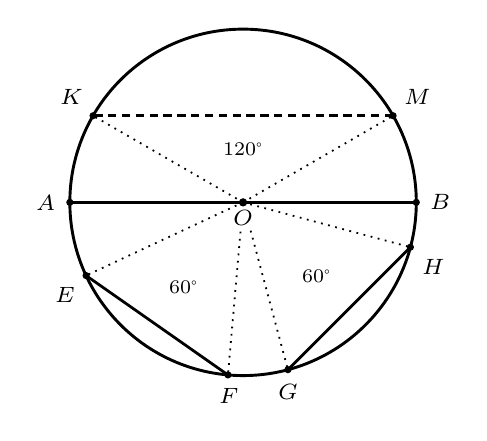
\begin{tikzpicture}[x=1cm, y=1cm, every node/.style={font=\footnotesize, text=black}]
      \coordinate (O) at (0,0);
      \pgfmathsetmacro{\R}{2.20}
      \draw[black, line width=1.05pt] (O) circle (\R);
      % Diameter AB (horizontal: 180 to 0)
      \coordinate (A) at (180:\R);
      \coordinate (B) at (0:\R);
      % Two 60-deg chords below: EF (-155 to -95) and GH (-75 to -15)
      \coordinate (E) at (-155:\R);
      \coordinate (F) at (-95:\R);
      \coordinate (G) at (-75:\R);
      \coordinate (H) at (-15:\R);
      % 120-deg chord above: MK (30 to 150) — also subtends major arc M-B-A-K = 240 deg!
      \coordinate (M) at (30:\R);
      \coordinate (K) at (150:\R);

      \draw[black, line width=1.15pt] (A) -- (B);
      \draw[black, line width=1.0pt] (E) -- (F) (G) -- (H);
      \draw[black, line width=1.05pt, densely dashed] (M) -- (K);
      \draw[black, line width=0.65pt, dotted] (O) -- (E) (O) -- (F) (O) -- (G) (O) -- (H) (O) -- (M) (O) -- (K);

      \fill[black] (O) circle (1.5pt) node[below=2pt, fill=white, inner sep=0.6pt] {$O$};
      \fill[black] (A) circle (1.3pt) node[left=1.5pt] {$A$};
      \fill[black] (B) circle (1.3pt) node[right=1.5pt] {$B$};
      \fill[black] (E) circle (1.3pt) node[below left=1pt] {$E$};
      \fill[black] (F) circle (1.3pt) node[below=1.5pt] {$F$};
      \fill[black] (G) circle (1.3pt) node[below=1.5pt] {$G$};
      \fill[black] (H) circle (1.3pt) node[below right=1pt] {$H$};
      \fill[black] (M) circle (1.3pt) node[above right=1pt] {$M$};
      \fill[black] (K) circle (1.3pt) node[above left=1pt] {$K$};

      \node[font=\scriptsize] at (-125:1.32) {$60^\circ$};
      \node[font=\scriptsize] at (-45:1.32) {$60^\circ$};
      \node[font=\scriptsize, fill=white, inner sep=0.6pt] at (90:0.68) {$120^\circ$};
    \end{tikzpicture}
  \end{tcolorbox}
\end{minipage}\hfill%
\begin{minipage}[t]{11.1cm}
  \vspace{0pt}
  \textbf{១. តារាង \en{POE} (ទស្សន៍ទាយមុនវាស់ រួចយកបន្ទាត់ក្រិតវាស់លើរូបខាងឆ្វេង)៖}\\[2pt]
  {\renewcommand{\arraystretch}{1.38}
  \begin{tabular}{|L{2.85cm}|C{1.45cm}|C{2.10cm}|C{3.85cm}|}
    \hline
    \cellcolor{panelgray}\textbf{ធ្នូនៃរង្វង់} & \cellcolor{panelgray}\textbf{មុំផ្ចិត} & \cellcolor{panelgray}\textbf{អង្កត់ធ្នូ} & \cellcolor{panelgray}\textbf{រង្វាស់វាស់បាន (\en{cm})} \\ \hline
    ធ្នូតូច $\arc{EF}$ & $60^\circ$ & $EF$ & \blank{1.6cm}$\unit{cm}$ \\ \hline
    ធ្នូតូច $\arc{GH}$ & $60^\circ$ & $GH$ & \blank{1.6cm}$\unit{cm}$ \\ \hline
    ធ្នូតូច $\arc{MK}$ & $120^\circ$ & $MK$ & \blank{1.6cm}$\unit{cm}$ \\ \hline
    កន្លះរង្វង់ $\arc{AMB}$ & $180^\circ$ & អង្កត់ផ្ចិត $AB$ & \blank{1.6cm}$\unit{cm}$ \\ \hline
    ធ្នូធំ $\arc{MFB}$--$K$ & $240^\circ$ & $MK$ & \blank{1.6cm}$\unit{cm}$ \\ \hline
  \end{tabular}}\\[3pt]
  \textbf{២. សំណួរវិភាគអន្ទាក់ការយល់ច្រឡំ (\en{Explain})៖}\\[1pt]
  $\bullet$ ធ្នូប៉ុនគ្នា $\arc{EF}=\arc{GH}=60^\circ \Rightarrow$ អង្កត់ធ្នូ $EF$ និង $GH$ \chkbox\ ប៉ុនគ្នា \;\chkbox\ មិនប៉ុនគ្នា\\[1pt]
  $\bullet$ ពេលមុំផ្ចិតកើនទ្វេដង ($60^\circ \to 120^\circ$) តើ $MK = 2 \times EF$ ($4.40\unit{cm}$) ដែរឬទេ?\\
  \hspace*{0.3cm}\chkbox\ ស្មើ $4.40\unit{cm}$ \quad \chkbox\ មិនស្មើទេ ($MK \approx \blank{1.1cm}\unit{cm} < 4.40\unit{cm}$)\\[1pt]
  $\bullet$ ធ្នូធំ $240^\circ$ វែងជាងកន្លះរង្វង់ $180^\circ$ តែអង្កត់ធ្នូ $MK$ \chkbox\ វែងជាង \;\chkbox\ ខ្លីជាង $AB$ !
\end{minipage}

\vspace{3pt}
\begin{tcolorbox}[
  enhanced, sharp corners, colback=white, colframe=black,
  boxrule=0.8pt, boxsep=1.5pt, top=2.0pt, bottom=2.0pt, left=5pt, right=5pt
]
  \begin{minipage}[c]{11.8cm}
    \textbf{៣. ឧទាហរណ៍ទី១ និងទី២ (ទំ.២០០) — និមិត្តសញ្ញាធ្នូ $\arc{AB}$ និងអង្កត់ធ្នូ $AB$ ៖}\\[2pt]
    $\bullet$ \textbf{ឧទាហរណ៍ទី១៖} បើធ្នូពីរត្រួតស៊ីគ្នា ($\arc{AB} = \arc{MN}$) នោះអង្កត់ធ្នូ $AB$ ត្រួតលើ $MN \Rightarrow AB = \blank{1.4cm}$ ។\\[2pt]
    $\bullet$ \textbf{ឧទាហរណ៍ទី២៖} ច្រាសមកវិញ បើអង្កត់ធ្នូ $AB = CD$ នោះចុងធ្នូត្រួតស៊ីគ្នា $\Rightarrow \arc{AB} = \blank{1.4cm}$ ។\\[2pt]
    $\bullet$ \textbf{សរុប POE៖} អង្កត់ធ្នូវែងបំផុតលើ $C(O, 2.20\unit{cm})$ គឺ \blank{2.2cm} ស្មើនឹង $2r = \blank{1.3cm}\unit{cm}$ ។
  \end{minipage}\hfill%
  \begin{minipage}[c]{6.4cm}
    \centering
    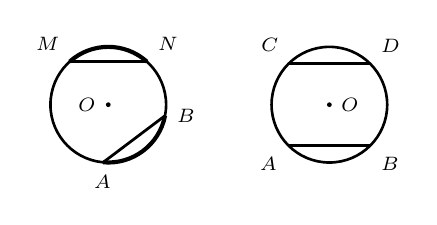
\begin{tikzpicture}[scale=0.72, every node/.style={font=\scriptsize, text=black}]
      \begin{scope}[shift={(0,0)}]
        \coordinate (O) at (1.2,1.1);
        \draw[black, line width=0.95pt] (O) circle (1.02);
        \draw[black, line width=1.0pt] ($(O)+(132:1.02)$) node[above left=0.5pt]{$M$} -- ($(O)+(48:1.02)$) node[above right=0.5pt]{$N$};
        \draw[black, line width=1.0pt] ($(O)+(-95:1.02)$) node[below=0.5pt]{$A$} -- ($(O)+(-11:1.02)$) node[right=0.5pt]{$B$};
        \draw[black, line width=1.5pt] ($(O)+(48:1.02)$) arc (48:132:1.02);
        \draw[black, line width=1.5pt] ($(O)+(-95:1.02)$) arc (-95:-11:1.02);
        \fill[black] (O) circle (1.2pt) node[left=1pt]{$O$};
      \end{scope}
      \begin{scope}[shift={(3.9,0)}]
        \coordinate (O) at (1.2,1.1);
        \draw[black, line width=0.95pt] (O) circle (1.02);
        \draw[black, line width=1.0pt] ($(O)+(135:1.02)$) node[above left=0.5pt]{$C$} -- ($(O)+(45:1.02)$) node[above right=0.5pt]{$D$};
        \draw[black, line width=1.0pt] ($(O)+(-135:1.02)$) node[below left=0.5pt]{$A$} -- ($(O)+(-45:1.02)$) node[below right=0.5pt]{$B$};
        \fill[black] (O) circle (1.2pt) node[right=1pt]{$O$};
      \end{scope}
    \end{tikzpicture}
  \end{minipage}
\end{tcolorbox}

% -------------------- ផ្នែក ខ (E3 Explain) --------------------
\secbox{ផ្នែក ខ \enbf{(E3 Explain)} ៖ សង្ខេបទ្រឹស្ដីបទ (ទំ.២០១) និងធនាគារហេតុផល \enbf{1--5}}{៦ នាទី \en{---} បំពេញប្រអប់ទ្រឹស្ដីបទ}

\begin{minipage}[t]{10.2cm}
  \vspace{2pt}
  $\bullet$ \textbf{ទ្រឹស្ដីបទទី១ (ទំ.២០១)៖} \blank{2.8cm} ជាអង្កត់ធ្នូដែល\textbf{វែងជាងគេ}នៅក្នុងរង្វង់មួយ ($AB > CD$) ។\\[4pt]
  $\bullet$ \textbf{ទ្រឹស្ដីបទទី២ (ទំ.២០១)៖} ក្នុងរង្វង់មួយ ឬរង្វង់ពីរប៉ុនគ្នា៖\\
  \hspace*{0.3cm}-- បើធ្នូប៉ុនគ្នា ($\arc{AB}=\arc{CD}$) នោះអង្កត់ធ្នូដែលសន្ធឹងធ្នូទាំងពីរក៏ \blank{2.3cm} ដែរ ។\\
  \hspace*{0.3cm}-- ច្រាសមកវិញ បើអង្កត់ធ្នូពីរប៉ុនគ្នា ($AB=CD$) នោះធ្នូដែលសន្ធឹងក្រោមអង្កត់ធ្នូទាំងពីរក៏ \blank{2.3cm} ដែរ ។\\[4pt]
  $\bullet$ \textbf{វិបាកប្រៀបធៀបធ្នូតូច៖} ក្នុងរង្វង់តែមួយ ចំពោះ\textbf{ធ្នូតូច}ពីរ ($<180^\circ$)៖\\
  \hspace*{0.3cm}$\arc{AB} > \arc{CD} \iff AB \;\blank{0.9cm}\; CD$ (ដាក់សញ្ញា $> , <$ ឬ $=$) ។
\end{minipage}\hfill%
\begin{minipage}[t]{8.4cm}
  \vspace{0pt}
  \begin{tcolorbox}[
    enhanced, sharp corners, colback=panelgray, colframe=black,
    boxrule=0.85pt, boxsep=1.5pt, top=3pt, bottom=3pt, left=5pt, right=5pt
  ]
    {\muol\fontsize{8.8pt}{12.5pt}\selectfont ធនាគារហេតុផល \enbf{(Warrant Bank)} សម្រាប់យោង៖}\\[3pt]
    {\fontsize{8.5pt}{12.8pt}\selectfont
    \cnum{1} \textbf{កាំរង្វង់តែមួយ៖} គ្រប់កាំនៃរង្វង់តែមួយស្មើគ្នា ($OA=OB=r$)\\
    \cnum{2} \textbf{វិសមភាពត្រីកោណ៖} ក្នុង $\tri{CDO}$ ផលបូក $OC+OD > CD$\\
    \cnum{3} \textbf{ត្រីកោណប៉ុនគ្នា (ជ.ជ.ជ)៖} ជ្រុង ៣ រៀងស្មើគ្នា $\Rightarrow$ មុំត្រូវគ្នាស្មើគ្នា\\
    \cnum{4} \textbf{សមមូលធ្នូ--អង្កត់ធ្នូ៖} $\arc{AB}=\arc{CD} \iff AB=CD$\\
    \cnum{5} \textbf{វិសមភាពធ្នូតូច៖} ចំពោះធ្នូតូច $\arc{AB}>\arc{CD} \iff AB>CD$}
  \end{tcolorbox}
\end{minipage}

\newpage
% ============================================================================
% ទំព័រទី ២ ៖ ផ្នែក គ (E4 Backward-Faded Proofs) + ផ្នែក ឃ (E5 Practice) + ផ្នែក ង (Exit & HW)
% ============================================================================
\secbox{ផ្នែក គ \enbf{(E4 Elaborate)} ៖ សម្រាយបញ្ជាក់បន្ថយជំនួយ (\enbf{Backward-Faded Proofs} ទំ.២០១)}{១០ នាទី \en{---} គូស \enbf{[tracing]} និងបំពេញជំហាន}

\begin{minipage}[t]{9.25cm}
  \begin{tcolorbox}[
    enhanced, sharp corners, colback=white, colframe=black,
    boxrule=0.8pt, boxsep=1.5pt, top=2.5pt, bottom=2.5pt, left=5pt, right=5pt
  ]
    \textbf{លំហាត់គំរូទី១ (ទំ.២០១ — បន្ថយជំនួយ ១ ជំហាន)៖}\\
    គេមានអង្កត់ផ្ចិត $AB$ និងអង្កត់ធ្នូ $CD$ ។ ស្រាយបញ្ជាក់ថា $AB > CD$ ។\\[2pt]
    \begin{minipage}[c]{3.15cm}
      \centering
      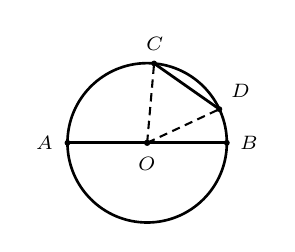
\begin{tikzpicture}[scale=0.88, every node/.style={font=\scriptsize, text=black}]
        \coordinate (O) at (0,0);
        \pgfmathsetmacro{\R}{1.15}
        \coordinate (A) at (180:\R);
        \coordinate (B) at (0:\R);
        \coordinate (C) at (85:\R);
        \coordinate (D) at (25:\R);
        \draw[black, line width=0.95pt] (O) circle (\R);
        \draw[black, line width=1.1pt] (A) -- (B);
        \draw[black, line width=1.0pt] (C) -- (D);
        \draw[black, line width=0.75pt, densely dashed] (O) -- (C) (O) -- (D);
        \fill[black] (O) circle (1.3pt) node[below=1.5pt] {$O$};
        \fill[black] (A) circle (1.2pt) node[left=1.5pt] {$A$};
        \fill[black] (B) circle (1.2pt) node[right=1.5pt] {$B$};
        \fill[black] (C) circle (1.2pt) node[above=1pt] {$C$};
        \fill[black] (D) circle (1.2pt) node[above right=1pt] {$D$};
      \end{tikzpicture}
    \end{minipage}\hfill%
    \begin{minipage}[c]{5.65cm}
      {\fontsize{8.5pt}{12.6pt}\selectfont
      $\bullet$ ភ្ជាប់ $O$ នឹង $C$ និង $O$ នឹង $D$ ។\\
      $\bullet$ ក្នុង $\tri{CDO}$ តាមហេតុផល \cnum{2}៖\\
      \hspace*{0.25cm}$OC + OD > CD \quad (i)$\\
      $\bullet$ តែតាម \cnum{1}៖ $OC+OD = r+r = \blank{1.0cm} \;(ii)$\\
      $\bullet$ តាម $(i)$ និង $(ii)$ បាន៖ $\blank{1.2cm} > \blank{1.2cm}$ ។}
    \end{minipage}
  \end{tcolorbox}
\end{minipage}\hfill%
\begin{minipage}[t]{9.25cm}
  \begin{tcolorbox}[
    enhanced, sharp corners, colback=white, colframe=black,
    boxrule=0.8pt, boxsep=1.5pt, top=2.5pt, bottom=2.5pt, left=5pt, right=5pt
  ]
    \textbf{លំហាត់គំរូទី២ (ទំ.២០១ — បន្ថយជំនួយ ២ ជំហាន)៖}\\
    ក្នុងរង្វង់ផ្ចិត $O$ មានអង្កត់ធ្នូ $MN=PQ$ ។ ស្រាយថា $\arc{MN}=\arc{PQ}$ ។\\[2pt]
    \begin{minipage}[c]{3.15cm}
      \centering
      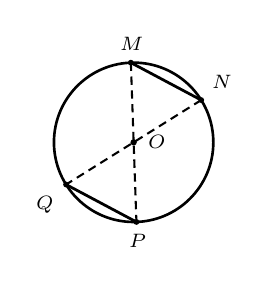
\begin{tikzpicture}[scale=0.88, every node/.style={font=\scriptsize, text=black}]
        \coordinate (O) at (0,0);
        \pgfmathsetmacro{\R}{1.15}
        \coordinate (M) at (92:\R);
        \coordinate (N) at (32:\R);
        \coordinate (P) at (-88:\R);
        \coordinate (Q) at (-148:\R);
        \draw[black, line width=0.95pt] (O) circle (\R);
        \draw[black, line width=1.0pt] (M) -- (N) (P) -- (Q);
        \draw[black, line width=0.75pt, densely dashed] (M) -- (P) (N) -- (Q);
        \fill[black] (O) circle (1.3pt) node[right=2pt] {$O$};
        \fill[black] (M) circle (1.2pt) node[above=1pt] {$M$};
        \fill[black] (N) circle (1.2pt) node[above right=1pt] {$N$};
        \fill[black] (P) circle (1.2pt) node[below=1pt] {$P$};
        \fill[black] (Q) circle (1.2pt) node[below left=1pt] {$Q$};
      \end{tikzpicture}
    \end{minipage}\hfill%
    \begin{minipage}[c]{5.65cm}
      {\fontsize{8.5pt}{12.6pt}\selectfont
      $\bullet$ ក្នុង $\tri{NOM}$ និង $\tri{POQ}$ មាន៖\\
      \hspace*{0.2cm}$OM=OP=ON=OQ$ (ហេតុផល \blank{0.6cm})\\
      \hspace*{0.2cm}និង $MN = PQ$ (\blank{1.8cm}) ។\\
      $\bullet$ នាំឱ្យ $\tri{NOM} \cong \tri{POQ}$ តាមករណី \blank{1.1cm}\\
      $\bullet$ វិបាក៖ $\ang{NOM} = \blank{1.3cm} \Rightarrow \arc{MN} = \arc{PQ}$ ។}
    \end{minipage}
  \end{tcolorbox}
\end{minipage}

\vspace{2pt}
\begin{tcolorbox}[
  enhanced, sharp corners, colback=white, colframe=black,
  boxrule=0.8pt, boxsep=1.5pt, top=2.0pt, bottom=2.0pt, left=5pt, right=5pt
]
  \begin{minipage}[c]{3.3cm}
    \centering
    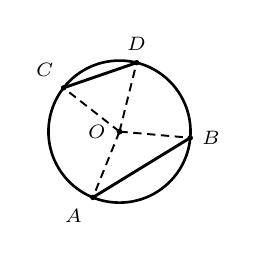
\begin{tikzpicture}[scale=0.82, every node/.style={font=\scriptsize, text=black}]
      \coordinate (O) at (0,0);
      \pgfmathsetmacro{\R}{1.10}
      \coordinate (A) at (-112:\R);
      \coordinate (B) at (-5:\R);
      \coordinate (C) at (142:\R);
      \coordinate (D) at (76:\R);
      \draw[black, line width=0.95pt] (O) circle (\R);
      \draw[black, line width=1.05pt] (A) -- (B) (C) -- (D);
      \draw[black, line width=0.7pt, densely dashed] (O) -- (A) (O) -- (B) (O) -- (C) (O) -- (D);
      \fill[black] (O) circle (1.3pt) node[left=1.5pt] {$O$};
      \fill[black] (A) circle (1.2pt) node[below left=0.5pt] {$A$};
      \fill[black] (B) circle (1.2pt) node[right=1pt] {$B$};
      \fill[black] (C) circle (1.2pt) node[above left=0.5pt] {$C$};
      \fill[black] (D) circle (1.2pt) node[above=1pt] {$D$};
    \end{tikzpicture}
  \end{minipage}\hfill%
  \begin{minipage}[c]{15.0cm}
    \textbf{លំហាត់គំរូទី៣ (ទំ.២០១ — បន្ថយជំនួយ ៣ ជំហាន)៖} ក្នុង $C(O,r)$ គេមានធ្នូតូច $\arc{AB} > \arc{CD}$ ។ ស្រាយថាអង្កត់ធ្នូ $AB > CD$ ៖\\
    $\bullet$ ក្នុង $\tri{AOB}$ និង $\tri{COD}$ មាន $OA = OB = OC = OD = r$ (តាមហេតុផល \blank{0.8cm}) ។\\
    $\bullet$ តែដោយធ្នូតូច $\arc{AB} > \arc{CD}$ នោះមុំផ្ចិតចន្លោះជ្រុងស្មើគ្នាផ្ទៀងផ្ទាត់ $\ang{AOB} \;\blank{0.8cm}\; \ang{COD} \Rightarrow$ អង្កត់ធ្នូ $\blank{1.2cm} > \blank{1.2cm}$ ។\\
    $\bullet$ \textbf{សំណួរត្រិះរិះ (\en{EIA 30s})៖} ហេតុអ្វីត្រូវបញ្ជាក់លក្ខខណ្ឌ «\textbf{ធ្នូតូច}»? ចម្លើយ៖ \blank{8.2cm}
  \end{minipage}
\end{tcolorbox}

% -------------------- ផ្នែក ឃ (E5 Practice / Proof) --------------------
\secbox{ផ្នែក ឃ \enbf{(E5 Evaluate)} ៖ ស្រាយបញ្ជាក់ដោយខ្លួនឯង (លំហាត់ទី២ ទំ.២០៤)}{៦.៥ នាទី \en{---} ប្រើវិធីដកធ្នូរួម}

\begin{minipage}[c]{4.8cm}
  \begin{tcolorbox}[
    enhanced, sharp corners, colback=white, colframe=black,
    boxrule=0.8pt, boxsep=1pt, top=2pt, bottom=2pt, left=2pt, right=2pt
  ]
    \centering
    {\fontsize{8.0pt}{10pt}\selectfont\textbf{លំហាត់ទី២ (ទំ.២០៤)៖ $\arc{AD}=\arc{CB}$}}\\[1pt]
    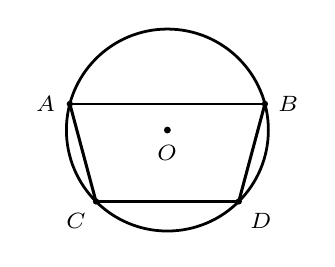
\begin{tikzpicture}[scale=0.95, every node/.style={font=\footnotesize, text=black}]
      \coordinate (O) at (0,0);
      \pgfmathsetmacro{\R}{1.35}
      \coordinate (A) at (165:\R);
      \coordinate (B) at (15:\R);
      \coordinate (C) at (-135:\R);
      \coordinate (D) at (-45:\R);
      \draw[black, line width=1.0pt] (O) circle (\R);
      \draw[black, line width=0.85pt] (A) -- (B) (C) -- (D);
      \draw[black, line width=1.1pt] (A) -- (C) (B) -- (D);
      \fill[black] (O) circle (1.3pt) node[below=2pt] {$O$};
      \fill[black] (A) circle (1.2pt) node[left=1.5pt] {$A$};
      \fill[black] (B) circle (1.2pt) node[right=1.5pt] {$B$};
      \fill[black] (C) circle (1.2pt) node[below left=1pt] {$C$};
      \fill[black] (D) circle (1.2pt) node[below right=1pt] {$D$};
    \end{tikzpicture}
  \end{tcolorbox}
\end{minipage}\hfill%
\begin{minipage}[c]{13.8cm}
  \textbf{ប្រធាន៖} គេឱ្យរង្វង់ $C(O,r)$ ដែលមានធ្នូ $\arc{AD} = \arc{CB}$ (មើលរូបខាងឆ្វេង) ។ ចូរស្រាយបញ្ជាក់ថា អង្កត់ធ្នូ $AC = BD$ ៖\\[3pt]
  $\bullet$ \textbf{ជំហានទី១ (បំបែកធ្នូជាផលបូក)៖} $\arc{AD} = \arc{AC} + \blank{1.5cm}$ និង $\arc{CB} = \arc{BD} + \blank{1.5cm}$ ។\\[4pt]
  $\bullet$ \textbf{ជំហានទី២ (ដកធ្នូរួមពីសម្មតិកម្ម $\arc{AD}=\arc{CB}$)៖} \blank{8.2cm}\\[4pt]
  $\bullet$ \textbf{ជំហានទី៣ (ទាញសន្និដ្ឋានតាមហេតុផលទី \blank{0.7cm})៖} ដូចនេះ អង្កត់ធ្នូ \blank{4.2cm} ។
\end{minipage}

% -------------------- ផ្នែក ង (E5 Exit Check & Homework) --------------------
\secbox{ផ្នែក ង \enbf{(E5 Exit Check \& Homework)} ៖ វាយតម្លៃរហ័ស \enbf{A--D} និងកិច្ចការផ្ទះ (ទំ.២០៤)}{៣.៥ នាទី \en{+} កិច្ចការផ្ទះ}

{\renewcommand{\arraystretch}{1.26}
\begin{tabular}{|C{0.7cm}|L{12.8cm}|C{2.4cm}|C{2.2cm}|}
  \hline
  \cellcolor{panelgray}\textbf{កូដ} & \cellcolor{panelgray}\textbf{អំណះអំណាងវិនិច្ឆ័យ (គូស \ding{51} ក្នុងប្រអប់ និងបញ្ជាក់លេខហេតុផល \cnum{1}--\cnum{5})} & \cellcolor{panelgray}\textbf{ជម្រើស} & \cellcolor{panelgray}\textbf{លេខហេតុផល} \\ \hline
  \enbf{A} & ក្នុងរង្វង់កាំ $r=7\unit{cm}$ គ្មានអង្កត់ធ្នូណាមួយអាចមានប្រវែងស្មើ $15\unit{cm}$ បានឡើយ ។ & \chkbox\ ត្រូវ \;\; \chkbox\ ខុស & \blank{1.4cm} \\ \hline
  \enbf{B} & បើធ្នូទីមួយមានរង្វាស់ដឺក្រេធំជាងធ្នូទីពីរ ២ ដង នោះអង្កត់ធ្នូទីមួយក៏វែងជាងអង្កត់ធ្នូទីពីរ ២ ដងដែរ ។ & \chkbox\ ត្រូវ \;\; \chkbox\ ខុស & \blank{1.4cm} \\ \hline
  \enbf{C} & ក្នុងរង្វង់តែមួយ បើអង្កត់ធ្នូពីរមានប្រវែងស្មើគ្នា ($AB=CD$) នោះធ្នូតូចទាំងពីរក៏ប៉ុនគ្នាដែរ ។ & \chkbox\ ត្រូវ \;\; \chkbox\ ខុស & \blank{1.4cm} \\ \hline
  \enbf{D} & ក្នុងរង្វង់តែមួយ ធ្នូធំ $250^\circ$ មានអង្កត់ធ្នូវែងជាងអង្កត់ផ្ចិត ($180^\circ$) ។ & \chkbox\ ត្រូវ \;\; \chkbox\ ខុស & \blank{1.4cm} \\ \hline
\end{tabular}}

\vspace{3pt}
\begin{tcolorbox}[
  enhanced, sharp corners, colback=white, colframe=black,
  boxrule=0.9pt, boxsep=1.5pt, top=2.5pt, bottom=2.5pt, left=6pt, right=6pt
]
  \begin{minipage}[c]{12.2cm}
    {\muol\fontsize{9.0pt}{13pt}\selectfont កិច្ចការផ្ទះ} \textbf{(សៀវភៅសិក្សាគោល ទំព័រ ២០៤ ៖ លំហាត់ទី៣ និង ទី៥)}\\[2pt]
    $\bullet$ \textbf{១. លំហាត់ទី៣ (ទំ.២០៤)៖} គេឱ្យរង្វង់ $C(O,r)$ មានអង្កត់ធ្នូ $AB = CD$ (រូបឆ្វេង) ។ ចូរស្រាយថា $\arc{AC} = \arc{BD}$ (\textit{តម្រុយ៖ ប្រើ \cnum{4} បាន $\arc{AB}=\arc{CD}$ រួចបូកអង្គទាំងពីរនឹងធ្នូរួម $\arc{BC}$}) ។\\[2pt]
    $\bullet$ \textbf{២. លំហាត់ទី៥ (ទំ.២០៤)៖} គេឱ្យរង្វង់ $C(O,r)$ មានអង្កត់ធ្នូ $AB = CD$ (រូបស្ដាំ) ។ ចូរបង្ហាញថា $\arc{BD} = \arc{AC}$ ។
  \end{minipage}\hfill%
  \begin{minipage}[c]{5.9cm}
    \centering
    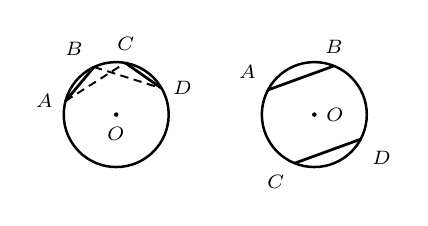
\begin{tikzpicture}[scale=0.68, every node/.style={font=\scriptsize, text=black}]
      \begin{scope}[shift={(0,0)}]
        \coordinate (O) at (1.15,1.05);
        \draw[black, line width=0.9pt] (O) circle (0.98);
        \draw[black, line width=1.0pt] ($(O)+(165:0.98)$) node[left=0.5pt]{$A$} -- ($(O)+(115:0.98)$) node[above left=0.5pt]{$B$};
        \draw[black, line width=1.0pt] ($(O)+(80:0.98)$) node[above=0.5pt]{$C$} -- ($(O)+(30:0.98)$) node[right=0.5pt]{$D$};
        \draw[black, line width=0.7pt, densely dashed] ($(O)+(165:0.98)$) -- ($(O)+(80:0.98)$) ($(O)+(115:0.98)$) -- ($(O)+(30:0.98)$);
        \fill[black] (O) circle (1.2pt) node[below=1pt]{$O$};
      \end{scope}
      \begin{scope}[shift={(3.7,0)}]
        \coordinate (O) at (1.15,1.05);
        \draw[black, line width=0.9pt] (O) circle (0.98);
        \draw[black, line width=1.0pt] ($(O)+(152:0.98)$) node[above left=0.5pt]{$A$} -- ($(O)+(68:0.98)$) node[above=0.5pt]{$B$};
        \draw[black, line width=1.0pt] ($(O)+(-112:0.98)$) node[below left=0.5pt]{$C$} -- ($(O)+(-28:0.98)$) node[below right=0.5pt]{$D$};
        \fill[black] (O) circle (1.2pt) node[right=1pt]{$O$};
      \end{scope}
    \end{tikzpicture}
  \end{minipage}
\end{tcolorbox}

\end{document}
